\chapter{Détails sur l'implémentation}
\section{Représentation du modèle}

\subsection{Les classes}
\subsubsection{Parcours}
Comme expliqué au chapitre précédent un parcours est constitué de plusieurs trajets. Donc la classe  \verb! Parcours! possédera une liste de trajets. Il regroupe également des informations qui lui sont propres tel qu'un nom et un identifiant. On remarquera également qu'un parcours possède un trajet de référence. Ce trajet est cruciale car il permettra la comparaison avec le trajet qui est effectué. Comme celui-ci pourra être modifié, on le représentera dans la classe  \verb! Parcours! par son identifiant. On ajoutera à cette classe tout un tas d'attributs servant à déterminer le meilleur temps, la vitesse moyenne, la vitesse maximale sur l'ensemble des trajets effectués.

\subsubsection{Trajet}
La classe  \verb! Trajet! représente le chemin qu'un utilisateur emprunte lorsqu'il effectue une course. On y retrouve une liste de points ( \verb! Location!) nécessaire à la visualisation du trajet ainsi qu'à la comparaison avec le trajet de référence. On gardera également des informations concernant la date à laquelle le trajet a été réalisé ainsi qu'un identifiant pour faciliter le stockage en base. Un trajet possède également une distance ainsi qu'un temps total. Ces deux attributs sont modifiés lors de l'ajout d'un point via la méthode \verb!addLocation! (détaillée dans l'Annexe \ref{Annexe1}) et permettent le calcul de la vitesse moyenne.

\subsubsection{Location}
Lors de implémentation du modèle, nous avions créé une classe Point permettant de stocker la latitude, la longitude et la date à laquelle le point est captée. Nous avions également établie la formule permettant de calculer la distance entre deux points (voir l'Annexe \ref{Annexe2}). Mais après avoir fait des recherches sur le fonctionnement du GPS sous Android, nous nous sommes aperçu que le \verb!LocationManager! retournait des objets \verb!Location! qui contiennent des attributs pour la latitude, la longitude et la date. De plus, une méthode \verb!distanceTo(Location l)! permet de calculer la distance entre deux points géolocalisés. 

\subsection{Le diagramme de classe}
Afin de résumer les parties précédentes, nous avons élaboré un diagramme de classes (Figure \ref{Diagramme de classes})
\begin{img}
  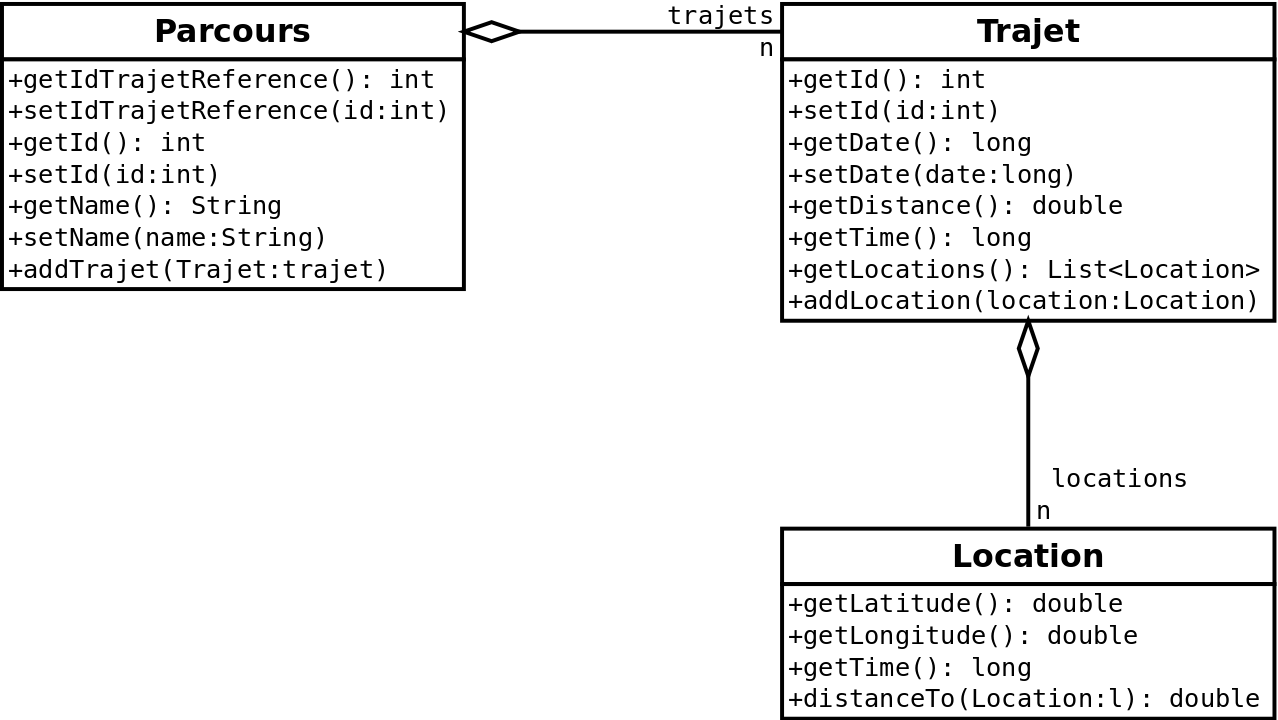
\includegraphics[scale=0.5]{img/DiagrammeDeClasse.png}
  \caption{Diagramme de classes}
  \label{Diagramme de classes}
\end{img}